\section{Tablas}

\begin{figure}[H]
    \centering
    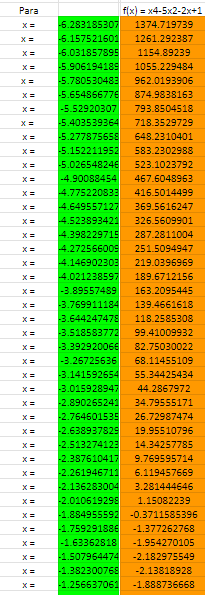
\includegraphics[width=2.13542in,height=6.19792in]{media/image23.png}
    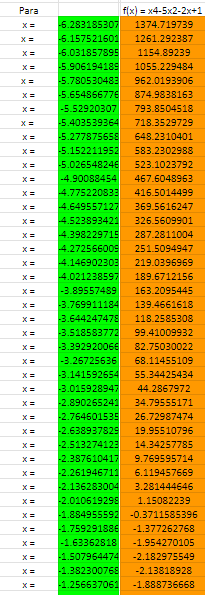
\includegraphics[width=2.13542in,height=6.19792in]{media/image23.png}    
    \caption{Función original en el rango \(-2 \pi\) a \(2 \pi\)}
\end{figure}

En la tabla 1 podemos observar los valores para la función \(\operatorname{f}(x) = x^4-5x^2-2x+1\), graficada en el intervalo \(-2 \pi\) a \(2 \pi\), para el rango de valores \(x\) , que representa el intervalo anteriormente mencionado se utilizaron 100 muestras. La columna de color verde muestra el valor de x para cada punto del intervalo, la columna naranja muestra la función evaluada en el valor. Estos valores serán utilizados para graficar la función original y así compararla con la transformada de Fourier. Cabe resaltar que contra mayor sea la cantidad de valores en que se divida el intervalo mayor será la definición que se obtenga de la función al momento de graficar.

\begin{figure}[H]
    \centering
    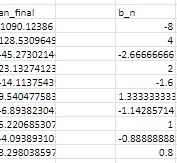
\includegraphics[width=1.84375in,height=1.69792in]{media/image1.png}
    \caption{Cálculo de \(a_n\) y \(b_n\)}        
\end{figure}

Una vez calculados los coeficientes \(a\) y \(b\) se pueden utilizar en la serie de Fourier para representar la función. Estos coeficientes representan la proyección de la función, normalizada por la longitud del periodo T.

\begin{figure}[H]
    \centering
    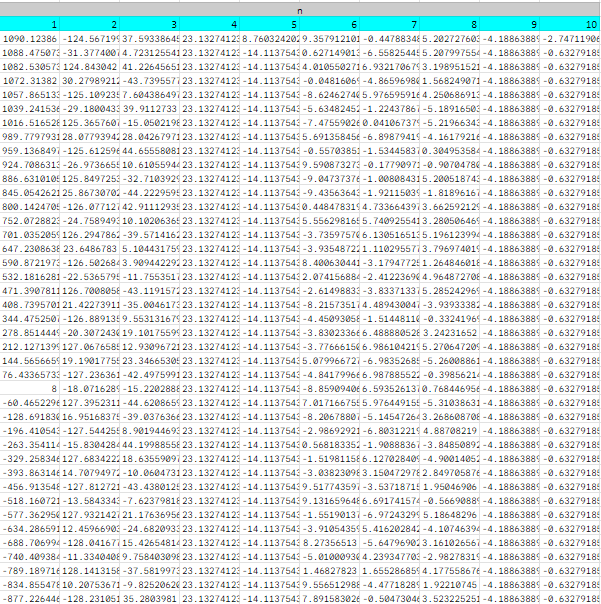
\includegraphics[width=5.5in,height=5.52745in]{media/image21.png}
    \caption{Matriz de cálculo de los coeficientes de la serie}
\end{figure}

En la tabla 3 se muestra el cálculo de los coeficientes de la serie de Fourier, cada columna (1-10), representa el cálculo de un coeficiente, los coeficientes están dados por la fórmula de series de Fourier, en donde hay que calcular \(a_n\) y \(b_n\) para cada valor de n, en este caso n siendo el intervalo 1-10, idealmente se deberían calcular todos los coeficientes, pero en este caso por las limitaciones de Excel solo se tomó una pequeña cantidad. La suma de coeficientes llevada de n=0 - n=infinito; nos daría exactamente la función que buscamos modelar, debido a que no se calculan todos en esta práctica veremos solamente una aproximación a la función original. Estos valores posteriormente serán utilizados para graficarlos y comparar la función original con la transformada de Fourier.

\begin{figure}[H]
    \centering
    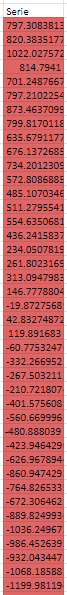
\includegraphics[width=0.69792in,height=6.19792in]{media/image28.png}
    \caption{Cálculo de la serie}
\end{figure}
En la Tabla 4 se muestran los resultados de los cálculos realizados que toman los valores de la serie de Fourier, se obtienen mediante la suma de los coeficientes previamente calculados, estos son utilizados para representar una función periódica como una suma de senos y cosenos.
